\chapter{Literature Review and Related Work}
\label{chap:relatedworks}

In this chapter, describe other solutions/research that address the
same topic as your project. If you are working on a software project, create a
list of alternative solutions and analyze them in the competitor analysis section.
If you are working on a research project, describe your related work research in
the literature review section.

\section{Competitor Analysis}
\label{section:competitor-analysis}

\begin{figure}[h]
    \centering
    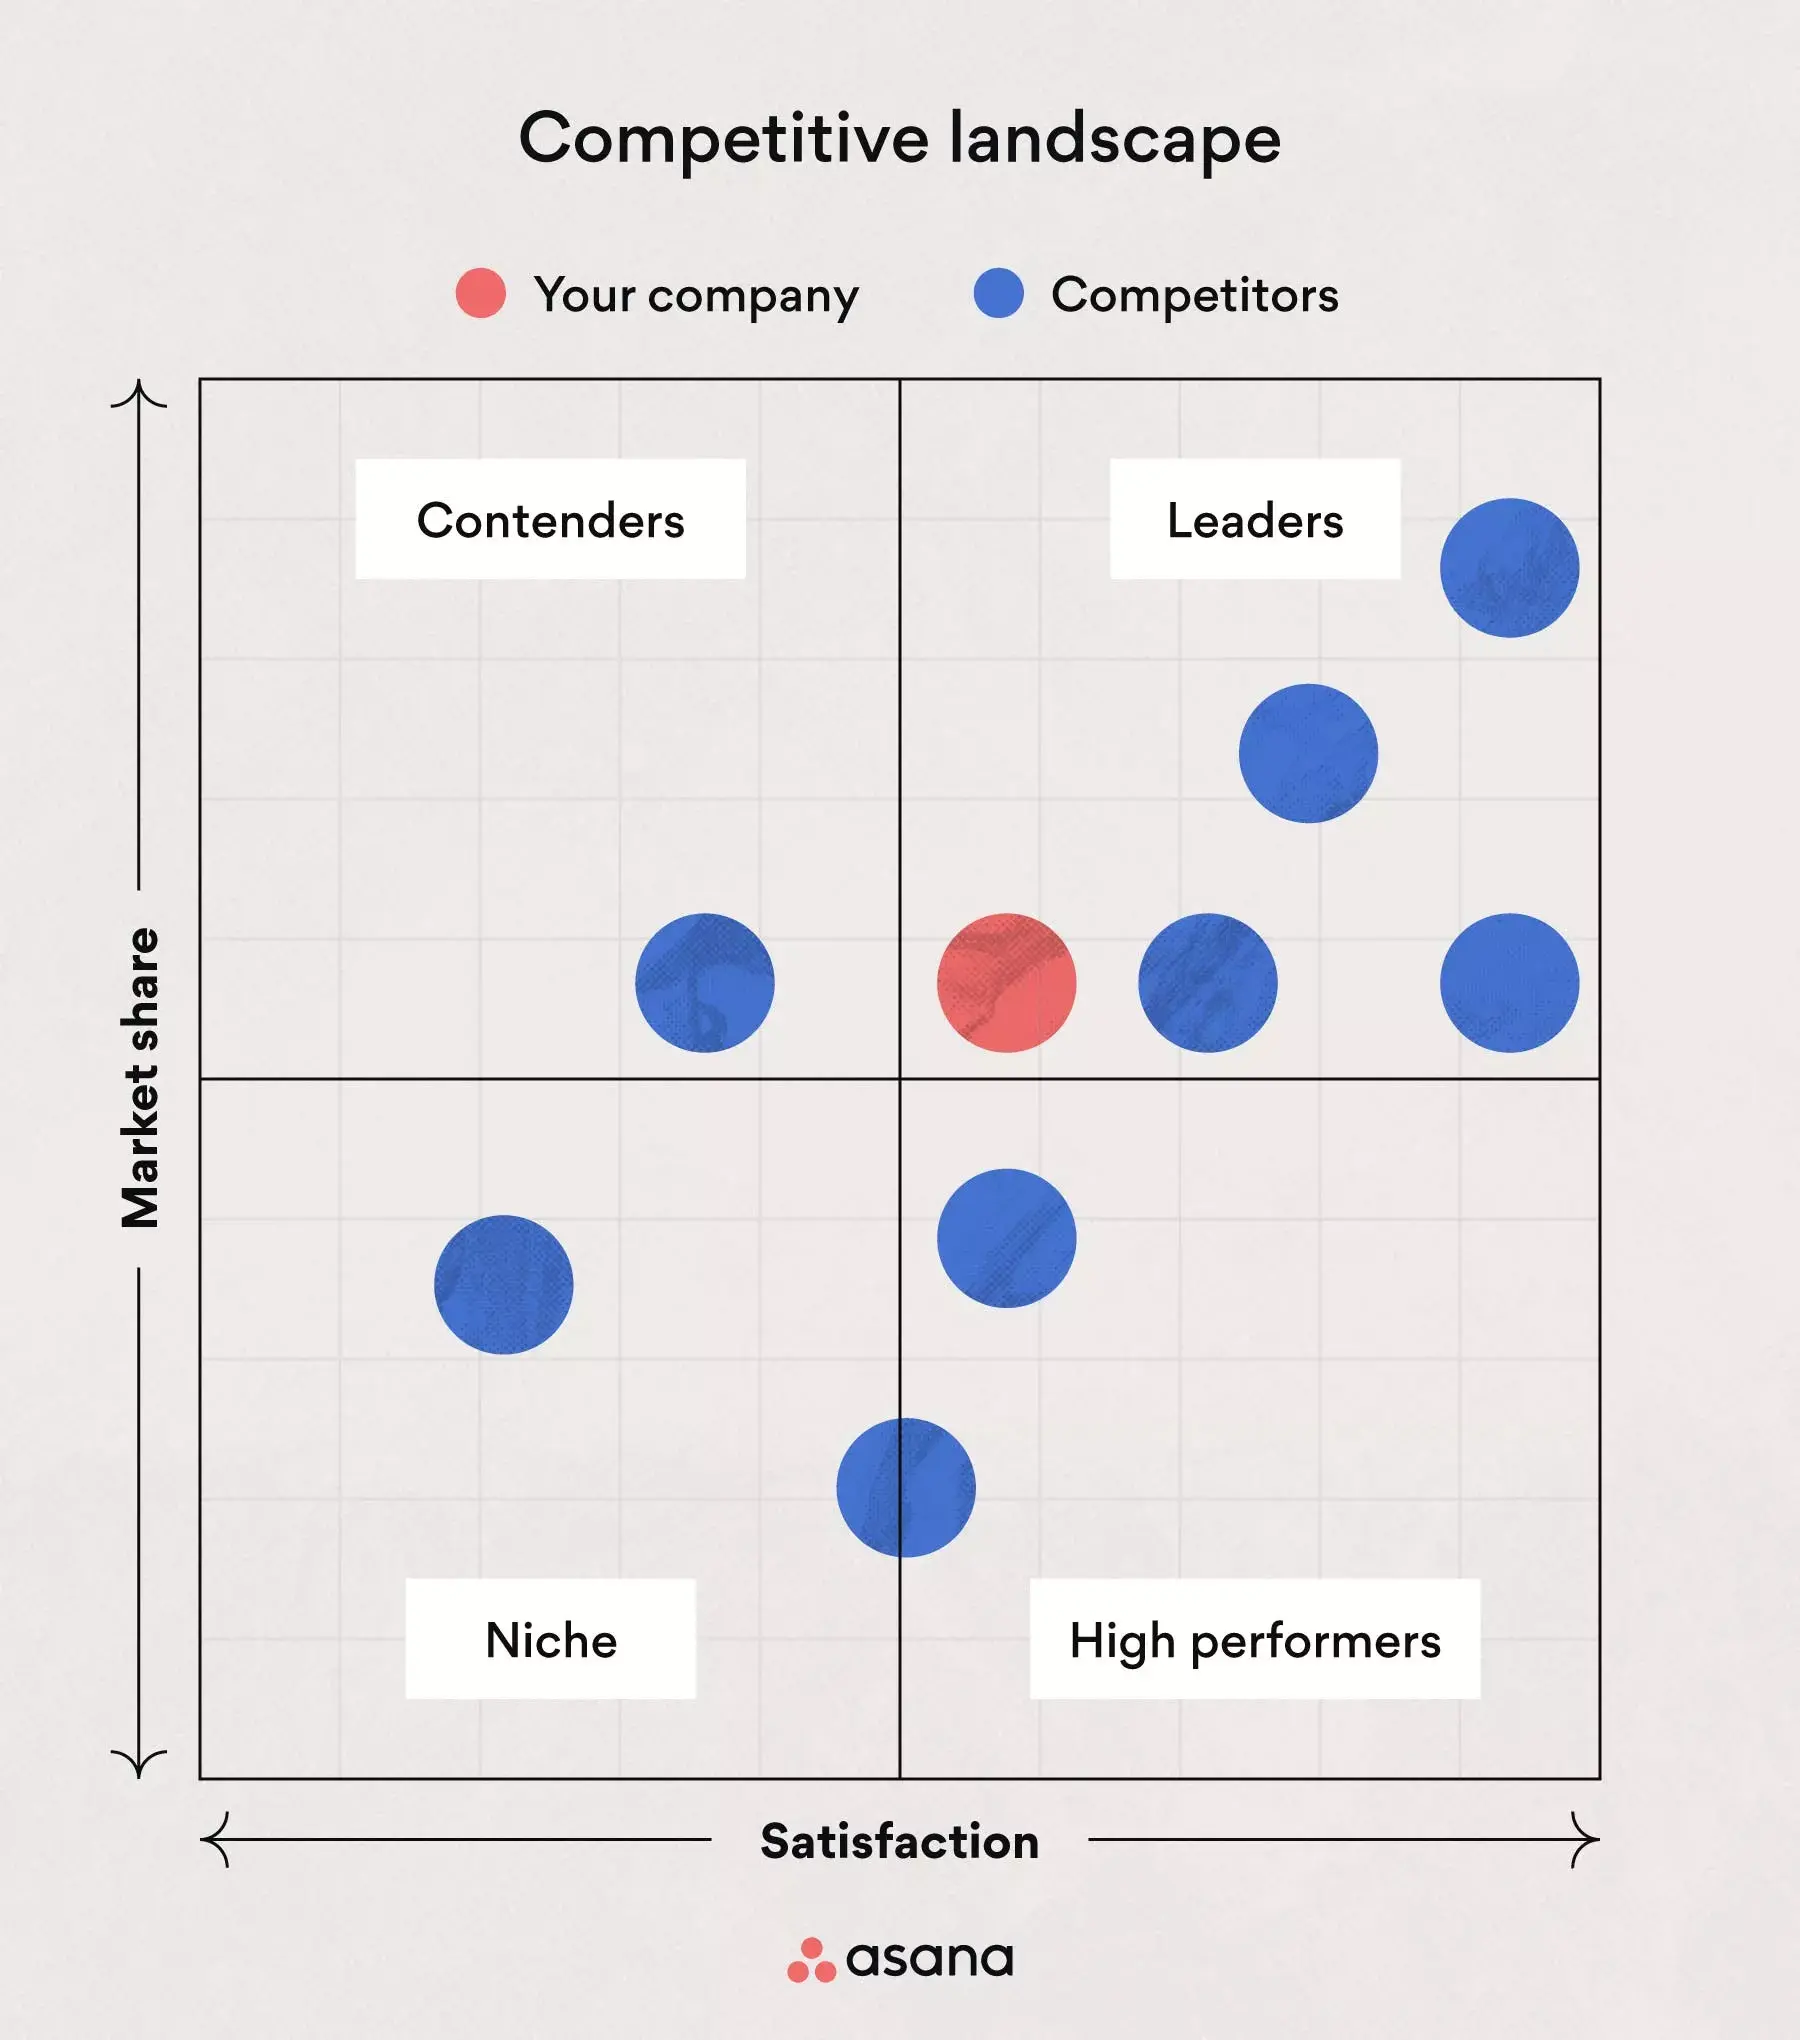
\includegraphics[width=0.5\textwidth]{examples/asana-competitive-landscape.jpg}
    \caption{Competitive Landscape by Asana}
\end{figure}

Refer to an article "How to create a competitive analysis (with
examples)" by Asana. You can use the Competitor Landscape (left image) or
Competitor Analysis Framework (right image) for your project.

\section{Literature Review}
\label{section:literature-review}

Parking management systems have been widely researched to address the challenges of finding vacant parking spaces, 
reducing user frustration when they cannot find available sparking spaces, and improving user convenience. 
This section reviews related studies and technologies that form the foundation for the KU Parking system.

A study by Barseghyan\cite{barseghyan2023parking} introduced a deep learning-based system for real-time parking occupancy detection using Convolutional Neural Networks (CNNs). 
The system processes video feeds from surveillance cameras to identify vacant parking spaces with high accuracy. 
By leveraging advanced image processing techniques, this approach eliminates the need for individual physical sensors, making it scalable and cost-effective. 
The use of CNNs aligns with KU Parking's adoption of YOLO (You Only Look Once) for vehicle detection, showcasing the efficacy of computer vision in parking management systems.

An et al.~\cite{an2022epsdnet} proposed EPSDNet, an intelligent detection method that directly uses deep learning 
for vehicle identification to implement parking detection without relying on lane line detection.
 Their approach constructs a TensorFlow deep learning platform for vehicle detection and determines the optimal time interval for 
 extracting video stream images based on vehicle arrival and departure patterns. 
 The system obtains parking space order and numbering through a combination of the TimSort algorithm and data layering method, 
 while parking space vacancy is judged via the indirect Monte Carlo method. Notably, 
 EPSDNet improves detection accuracy by ensuring greater distance between vehicles in the training dataset compared to those observed during detection. 
 This camera-based approach aligns with KU Parking's goal of utilizing existing surveillance infrastructure rather than installing costly sensor systems for each parking space.

Ciampi et al.~\cite{ciampi2022multicamera} developed a multi-camera system for vehicle counting in parking lots using edge-AI technology. 
Their approach employs a modified Mask R-CNN detector running on edge devices to locate vehicles, combined with a decentralized algorithm that uses homographic transformations to handle overlapping camera views. 
Testing on the CNRPark-EXT dataset showed significant improvement over single-camera methods, with a mean relative error of just 1.6\%. 
The system processes data at the source rather than relying on central servers, reducing network bandwidth requirements. 
This research supports KU Parking's strategy of utilizing existing camera infrastructure with computer vision rather than installing dedicated sensors, 
while providing the flexibility needed for distributed campus parking areas.

Traditional parking systems often rely on physical sensors installed at each parking spot to detect occupancy. 
While effective, these systems are expensive to install and maintain, especially in large-scale environments such as university campuses. 
KU Parking addresses these limitations by utilizing existing surveillance cameras integrated with cloud-based image processing, 
significantly reducing installation costs while maintaining accuracy.

By building upon these technologies and methodologies, KU Parking aims to deliver an innovative, scalable, and user-friendly solution tailored to the needs of Kasetsart University's Bangkhen Campus.